% Deliverable 3 results. All measurements in this section were supplied by the
% completed D3 experiment logs, NOT taken from the older D3 branch.
% This file is intentionally separate from report/sections/phase5_results.tex.
\clearpage
\section{Phase 5: Comparative Analysis and Failure Diagnostics}
\label{sec:d3-phase5}

\subsection{Research Questions and Evaluation Protocol}
The final experiment addresses four questions: (RQ1) Does the fully trained
PyTorch heuristic reduce node expansions relative to Manhattan A$^\ast$?
(RQ2) How often does it retain optimal path costs?
(RQ3) Which maze properties and prediction-field defects accompany poor search
performance? (RQ4) Which feature groups matter when a comparable neural
regressor is trained with fewer inputs?

The held-out test split comprises 282 entire mazes (140 Backtracker and 142
Perlin), with grid sizes 20, 40, 60, 80, and 100. The numbers of test mazes at
these sizes are 56, 58, 67, 45, and 56, respectively. Both search methods
solve the same maze instances, so comparisons are paired by maze. The primary
search results in this section use \emph{the corrected Deliverable 2 PyTorch
checkpoint}, not the scikit-learn fallback used for the older Phase~4
benchmark. The search experiment uses the raw neural field with scaling
$\alpha=1.0$ and the same A$^\ast$ engine and tie-breaking as Manhattan.

\subsection{Trained Model Provenance}
The primary checkpoint is
\texttt{models/neural\_heuristic\_seed42.pt} (seed 42; 29 inputs; hidden
layers 256--256--128; dropout 0.1; regression output plus 10 distance bins).
It contains 107,787 parameters and was configured for up to 20 epochs.
Training stopped after 11 epochs; epoch 6 gave the best validation MAE of
$0.05161$ in normalized $h^\ast/N$ units. The checkpoint SHA-256 is
\texttt{86565d7891f40b81}\allowbreak\texttt{3879e1fe0da3c231}\allowbreak\texttt{85ae2b1dc2fa2b0e}\allowbreak\texttt{624690b2b94d6da4}.
The original D2 training also recorded replicate runs with seeds 43 and 44,
but the new D3 search comparison is only for the seed-42 checkpoint. It would
be incorrect to describe this checkpoint as a one-epoch smoke-test artifact.

\subsection{RQ1: Paired Search Efficiency}
\label{sec:d3-paired}
\begin{table}[H]
\centering
\small
\begin{tabular}{lr}
\toprule
\textbf{Measure} & \textbf{282 held-out mazes} \\
\midrule
Manhattan mean nodes expanded & 180.79 \\
PyTorch neural mean nodes expanded & 498.58 \\
Mean paired difference (neural $-$ Manhattan) & $+317.78$ \\
95\% bootstrap CI for mean paired difference & $[+256.52,+385.52]$ \\
Ratio of overall mean expansions & $2.76\times$ \\
Mean of per-maze expansion ratios & $3.85\times$ \\
Mazes where neural expands fewer / same / more & 15 / 4 / 263 \\
Wilcoxon signed-rank $p$-value & $5.81\times10^{-43}$ \\
\bottomrule
\end{tabular}
\caption{Paired comparison of raw PyTorch neural A$^\ast$ and Manhattan A$^\ast$.
Lower expansion counts are better. The two ratio summaries use different
aggregation rules and should not be confused.}
\label{tab:d3-paired}
\end{table}

The neural method expands 317.78 additional nodes per maze on average, with a
paired-bootstrap 95\% interval entirely above zero. The Wilcoxon signed-rank
test rejects a zero-centered paired difference at conventional significance
levels. However, a small $p$-value establishes a statistical association in
this fixed benchmark, not a general causal explanation for search failure.
Neural A$^\ast$ improves expansion count on only 15 of the 282 mazes.

\subsection{RQ2: Path Quality and Optimality}
\label{sec:d3-optimality}
Neural A$^\ast$ returns an optimal path on 232 mazes (82.3\%) and a longer
path on 50 (17.7\%). Its mean optimality ratio, defined as neural path cost
divided by oracle shortest-path cost, is $1.00820$; this corresponds to an
average path-length excess of approximately 0.82\%. Manhattan A$^\ast$ has
mean optimality ratio $1.0$ in the recorded comparison. Thus, although the
learned search retains near-optimal mean path quality, it has no expansion
advantage on the full test split.

\subsection{Performance across Generators, Sizes and Densities}
\label{sec:d3-strata}
\begin{table}[H]
\centering
\small
\begin{tabular}{rrrrr}
\toprule
Grid size & Mazes & Manhattan nodes & Neural nodes & Mean maze ratio \\
\midrule
$20\times20$ & 56 & 30.18 & 49.41 & $1.76\times$ \\
$40\times40$ & 58 & 58.55 & 152.45 & $2.55\times$ \\
$60\times60$ & 67 & 152.96 & 394.93 & $4.02\times$ \\
$80\times80$ & 45 & 407.11 & 739.89 & $4.79\times$ \\
$100\times100$ & 56 & 367.04 & 1236.34 & $6.34\times$ \\
\bottomrule
\end{tabular}
\caption{Size-stratified search results. The last column averages each maze's
neural-to-Manhattan ratio and is not the ratio of the two mean columns.}
\label{tab:d3-size}
\end{table}

The disparity generally grows with grid size. By generator, the mean per-maze
ratio is approximately $3.72\times$ for Backtracker and $3.98\times$ for
Perlin, with higher expansion counts for neural search in both groups.
Density-stratified mean per-maze ratios also vary, but these group
comparisons are descriptive; generator, size, and obstacle-density effects
need not be independent. These results identify the larger mazes as an
especially important failure regime.

\subsection{RQ3: Error, Admissibility and Local Consistency}
\label{sec:d3-field}
The field-diagnostic analysis covers 911,949 reachable test cells. Relative
to exact remaining distances, the trained network has a mean absolute error
of 4.72 cells, an RMSE of 12.88 cells, and a mean signed error
(prediction minus truth) of $-2.78$ cells. In spite of this negative mean bias,
55.32\% of reachable-cell estimates exceed the exact distance; an overall
negative mean is compatible with frequent overestimates when underestimation
errors have greater magnitude.

On the 1,551,727 evaluated adjacent reachable-cell pairs, 755,169 pairs
(48.44\%) violate the unit-cost local consistency condition
$|h_\theta(u)-h_\theta(v)|\leq1$ for traversable neighbors. This shows the
learned field need not behave like the geometrically consistent Manhattan
heuristic. Such violations can contribute to less effective node ordering,
but their prevalence alone does not establish a specific causal mechanism.

Across mazes, Spearman correlation between the overestimation fraction and
the neural/Manhattan expansion ratio is about $\rho=0.563$ ($p<10^{-24}$).
The corresponding correlation for adjacent-pair inconsistency is
$\rho=-0.077$ ($p\approx0.198$), which is not statistically significant in
this analysis. Per-maze MAE has a weaker positive association with the
expansion ratio ($\rho\approx0.209$, $p\approx3.10\times10^{-7}$).
These exploratory associations suggest that field quality matters, but do
not demonstrate which errors independently cause additional expansions.

\begin{figure}[H]
\centering
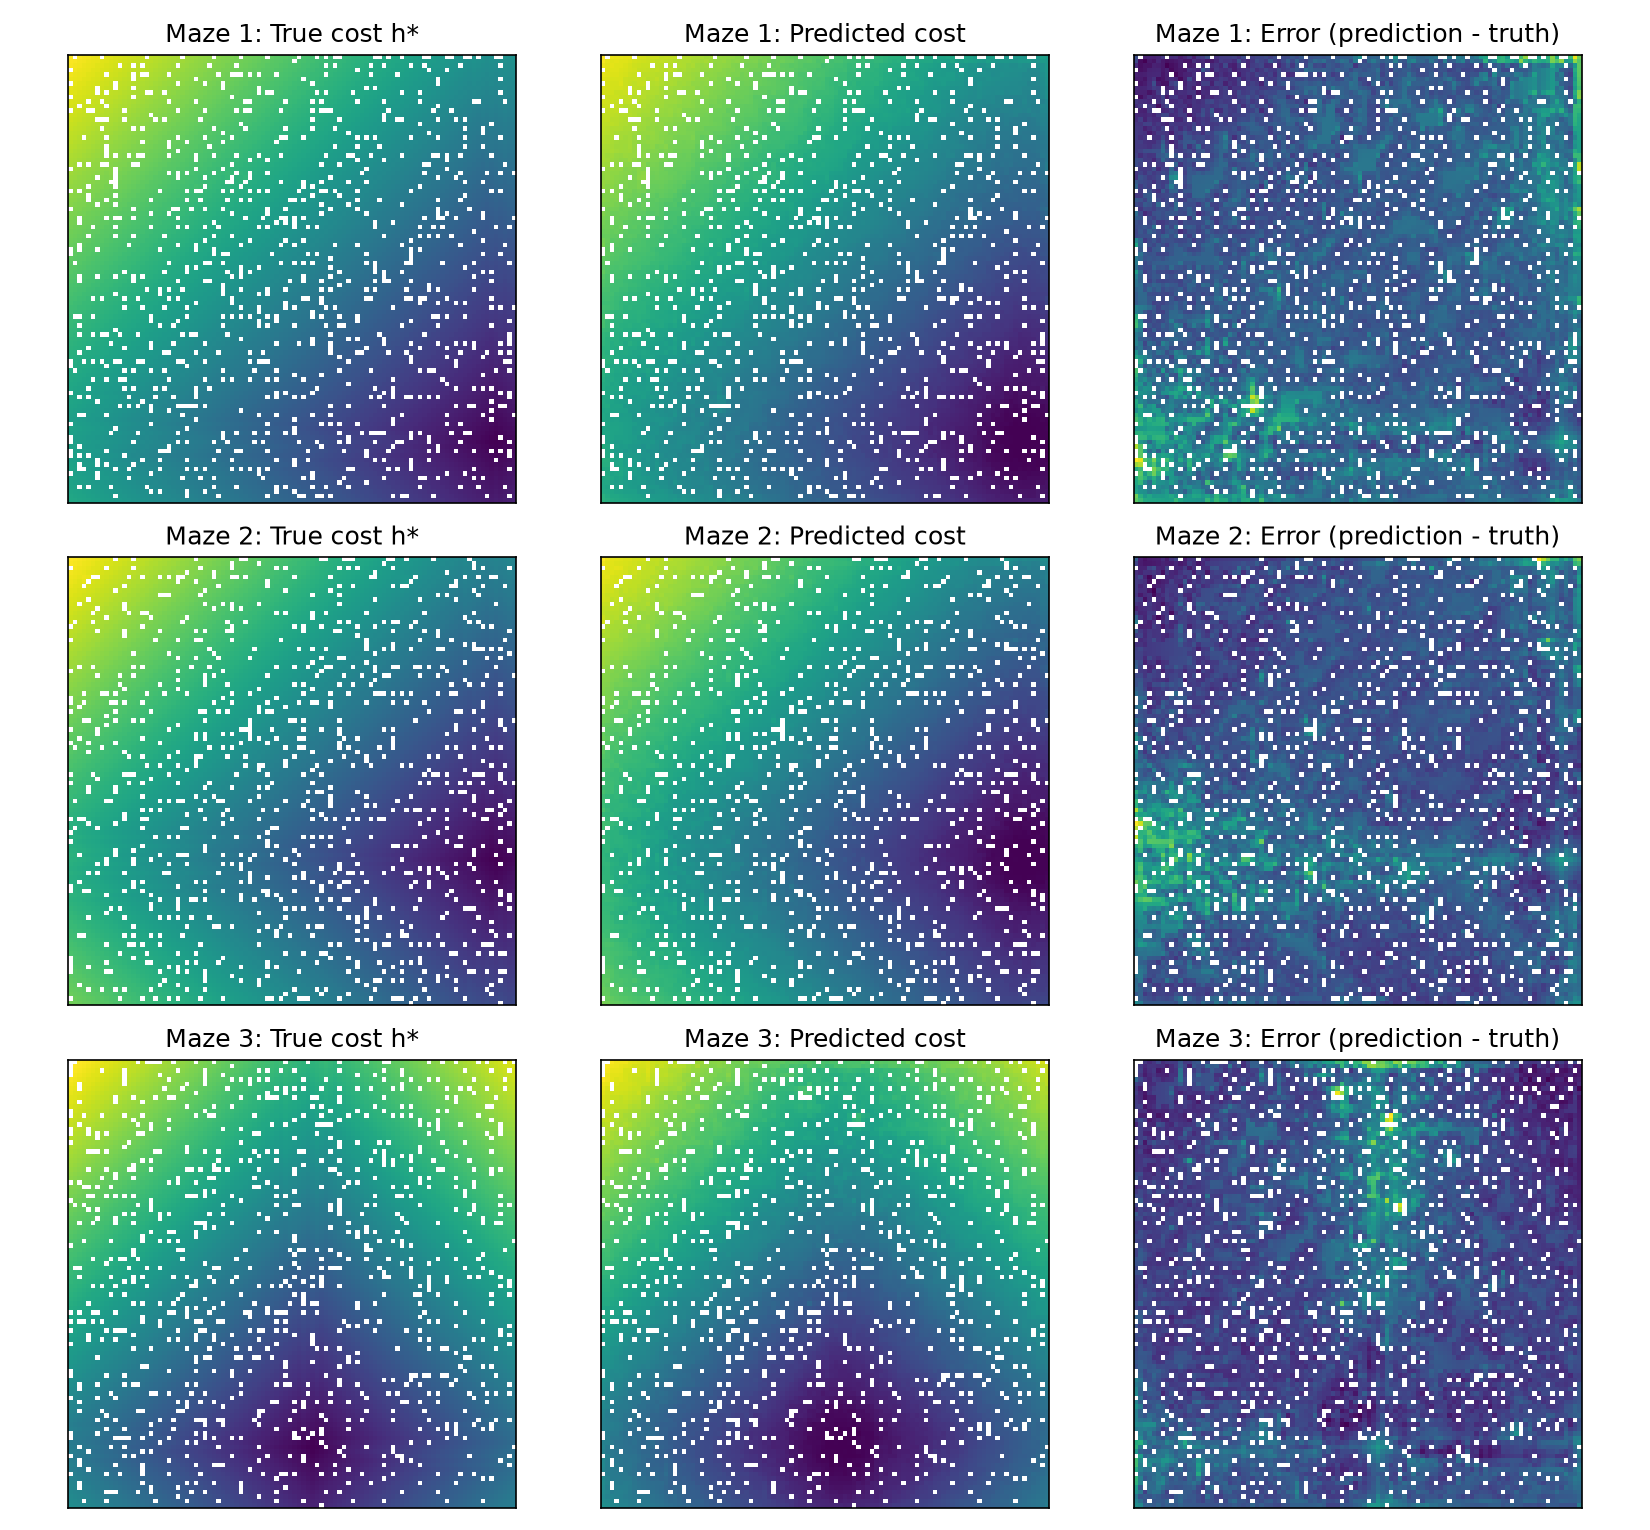
\includegraphics[width=0.92\textwidth]{figures/d3/prediction_fields.png}
\caption{Representative prediction-field visualization generated using the
corrected PyTorch checkpoint.}
\label{fig:d3-prediction-fields}
\end{figure}

\begin{figure}[H]
\centering
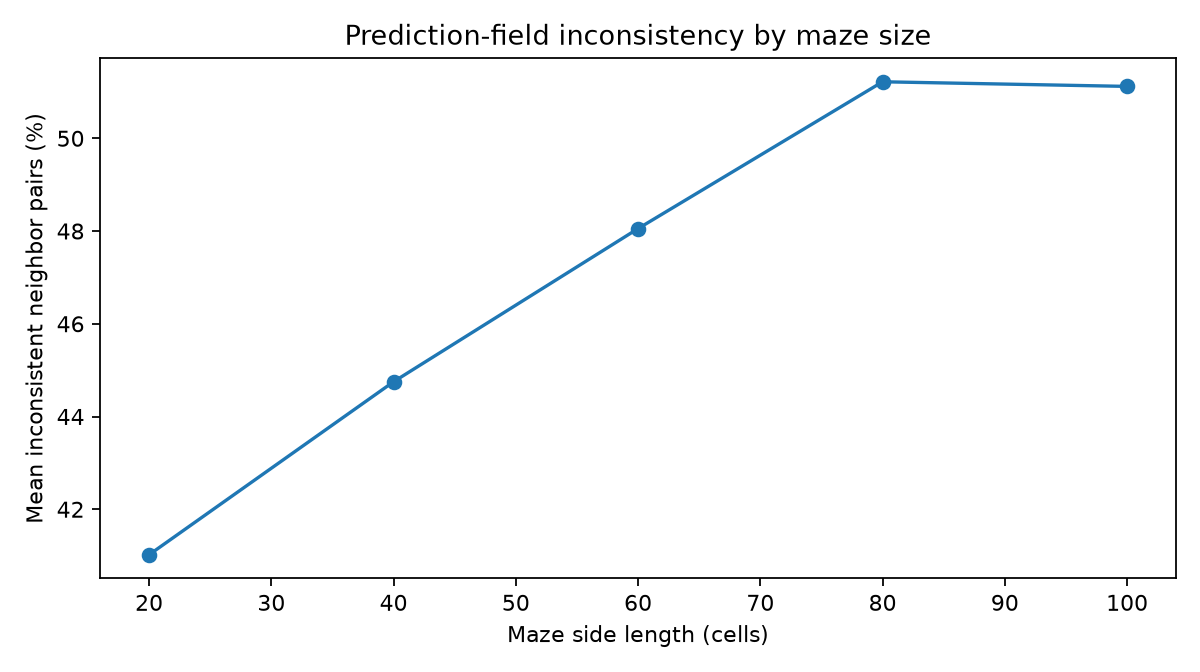
\includegraphics[width=0.78\textwidth]{figures/d3/inconsistency_by_size.png}
\caption{Adjacent-cell consistency diagnostics grouped by grid size.}
\label{fig:d3-inconsistency-size}
\end{figure}

\begin{figure}[H]
\centering
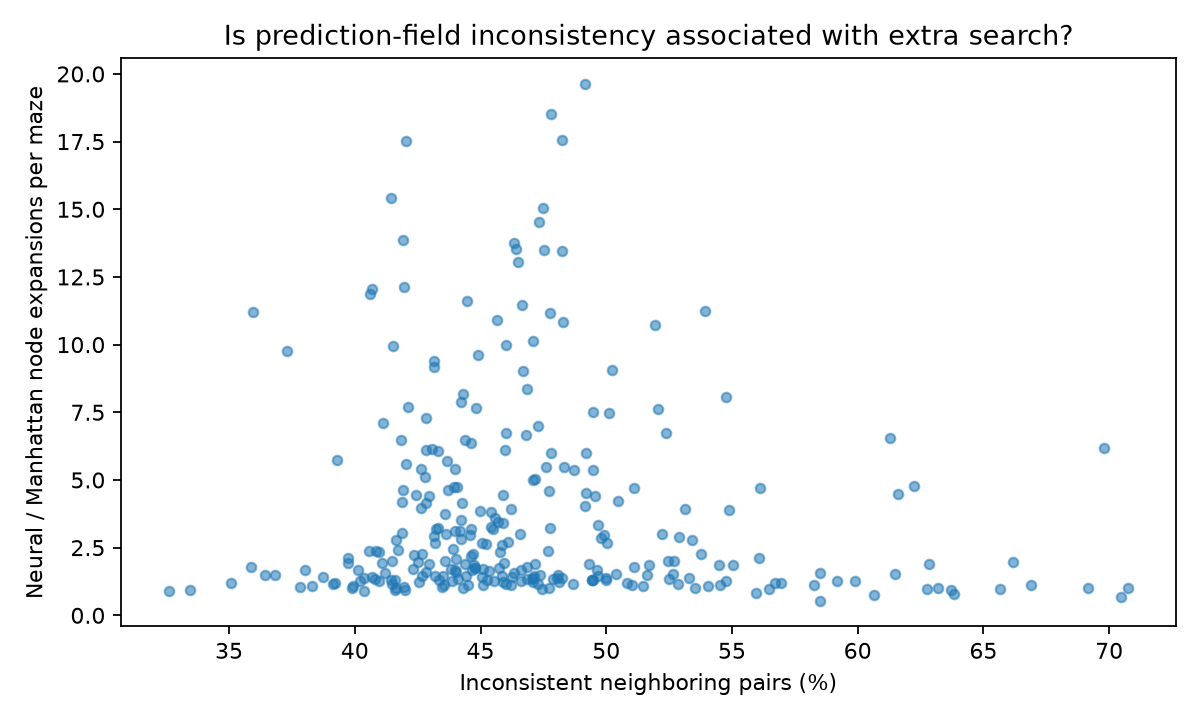
\includegraphics[width=0.78\textwidth]{figures/d3/inconsistency_vs_expansion.png}
\caption{Per-maze consistency and search-expansion relationship.}
\label{fig:d3-inconsistency-expansion}
\end{figure}

\begin{figure}[H]
\centering
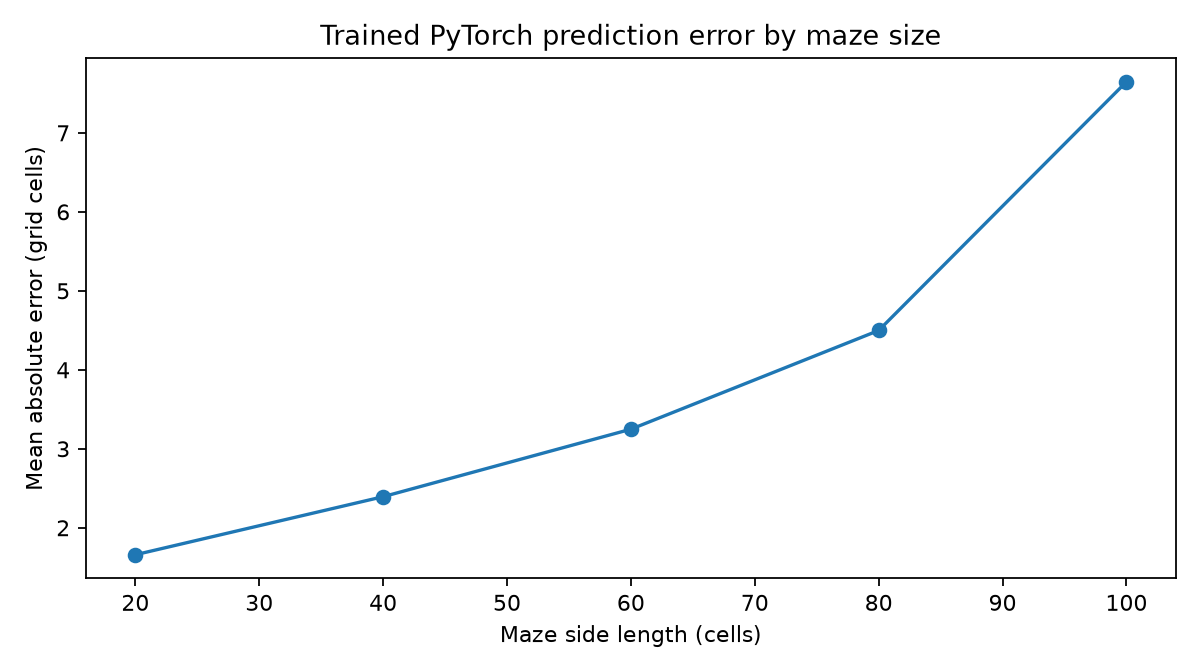
\includegraphics[width=0.78\textwidth]{figures/d3/prediction_mae_by_size.png}
\caption{Cell-level absolute prediction errors by maze size.}
\label{fig:d3-mae-size}
\end{figure}

\subsection{RQ4: Feature-Ablation Study}
\label{sec:d3-features}
Five reduced-feature scikit-learn MLP regressors were trained separately with
seed 42, 30,000 sampled training cells per variant, up to 50 training
iterations, and cell evaluation on 30,000 held-out test cells. All variants
were compared on the same 282 held-out mazes. \emph{These are ablation models;
none is the 256--256--128 PyTorch checkpoint used in RQ1--RQ3.}

\begin{table}[H]
\centering
\small
\begin{tabular}{lrrr}
\toprule
Feature set & Features & Cell MAE ($h^\ast/N$) & Mean A$^\ast$ nodes \\
\midrule
All inputs & 29 & 0.0774 & 558.58 \\
Without wall window & 4 & 0.0770 & 449.76 \\
Goal offsets only & 2 & 0.0786 & 358.58 \\
Without goal offsets & 27 & 0.2976 & 2044.11 \\
Without coordinates & 27 & 0.0795 & 561.06 \\
\midrule
Manhattan (no learned model) & --- & --- & 180.79 \\
\bottomrule
\end{tabular}
\caption{Independent scikit-learn feature ablations; lower is better.
The ablation MAE values are not directly interchangeable with the primary
PyTorch validation MAE because they concern different model runs and splits.}
\label{tab:d3-feature}
\end{table}

The goal-offset-only variant expands fewer nodes than the full-feature
ablation model, even though their prediction MAEs are similar. Removing
relative goal offsets severely damages both regression and search results.
Nevertheless, none of the learned variants beats Manhattan on mean node
expansions. The study indicates that minimizing cell-level prediction error
is not sufficient to optimize a search procedure, which also depends on the
spatial structure and ordering induced by the heuristic field.

\subsection{Limitations, Reproducibility and Interpretation}
\label{sec:d3-limitations}
The experiments use static, procedurally generated, four-connected mazes;
there is no measured transfer to dynamic obstacles or real-world robotic
systems. The main PyTorch search study evaluates a single trained checkpoint
(seed 42), so robustness across independently trained seeds remains an open
question. The separate feature-ablation results do not isolate the effect
of deleting features from the \emph{same} trained PyTorch architecture:
they retrain a different scikit-learn regressor with a fixed small sample.
Tests of several associations are exploratory rather than preregistered.
Runtime comparisons were not reported in the new primary D3 search summary,
so no new PyTorch latency advantage or disadvantage is claimed here.

The full benchmark and diagnostics can be reproduced using the repository's
existing cleaned data, split manifest and seed-42 checkpoint. Evidence is
stored under \texttt{results/analysis/d3/full\_test\_raw/} (paired A$^\ast$
results, failure summary and field diagnostics), under
\texttt{results/analysis/d3/feature\_ablation\_full/}, and in
\texttt{figures/d3/}. The checkpoint hash should be checked against the
metadata above before re-running experiments. The pre-existing D2 fallback
benchmark remains a separate experiment and is not overwritten by D3.

\subsection{Phase 5 Conclusion}
Across all 282 held-out mazes, the corrected, trained PyTorch model preserves
near-optimal mean path costs but expands significantly more nodes than
Manhattan. Larger maps show larger relative expansion penalties, and the
neural field frequently overestimates true distances and violates local
consistency. Overestimation rates correlate with poor search efficiency,
although these descriptive correlations do not establish causal mechanisms.
Feature ablations reinforce the finding that a low regression MAE need not
produce an effective A$^\ast$ heuristic. The central hypothesis of fewer
expansions under neural guidance is \emph{not supported} by these experiments.
